\documentclass[11pt]{article}
\usepackage[margin=1in]{geometry}
\usepackage{graphicx}
\usepackage{amsmath}
\usepackage{amssymb}
\usepackage{float}
\usepackage{subcaption}

\title{July 8, 2021 Meeting Agenda}

\begin{document}
\maketitle

\section{Discussion about what assignment types to include}
  To differentiate between the calendar assignment types (e.g. single assignment, multiple assignment, etc) I have decided to call the work designation on the calendar (e.g. GS or GS CP) "work type". When trying to think about what to do about work types other than GS, I realized I didn't have a good idea of how the average pleas processed per day varied across these designations. I plotted it because I think this could be useful when thinking about what to do.

  \begin{figure}[H]
    \centering
    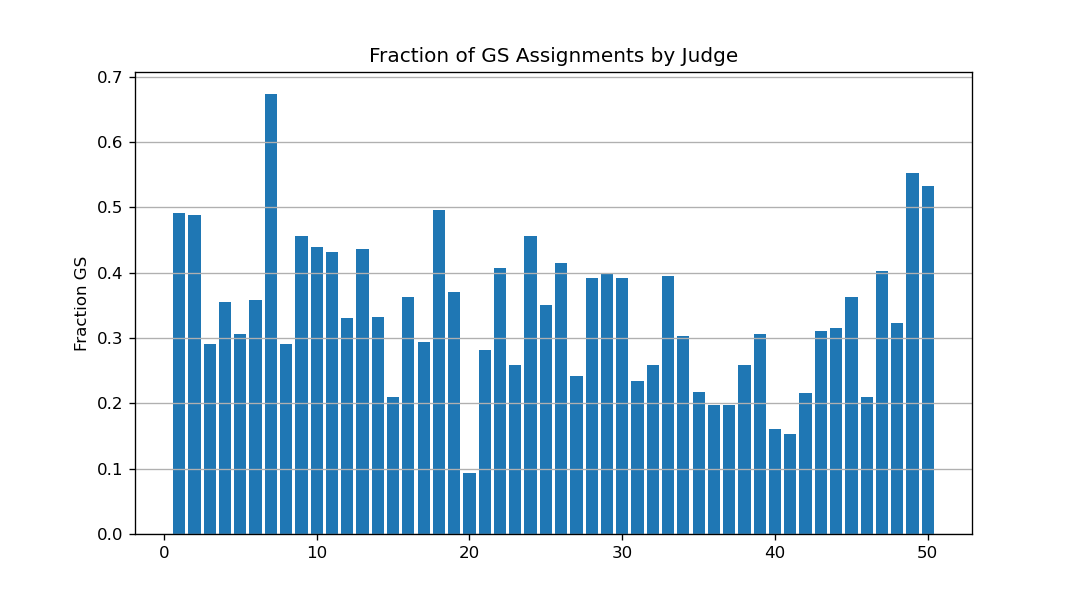
\includegraphics[width=0.75\textwidth]{../../../output/figures/Exploration/fraction_gs_by_judge.png}
    \caption{Fraction of GS-only Assignments by Judge}
    \label{fig-frac-gs}
  \end{figure}

  \begin{figure}[H]
    \centering
    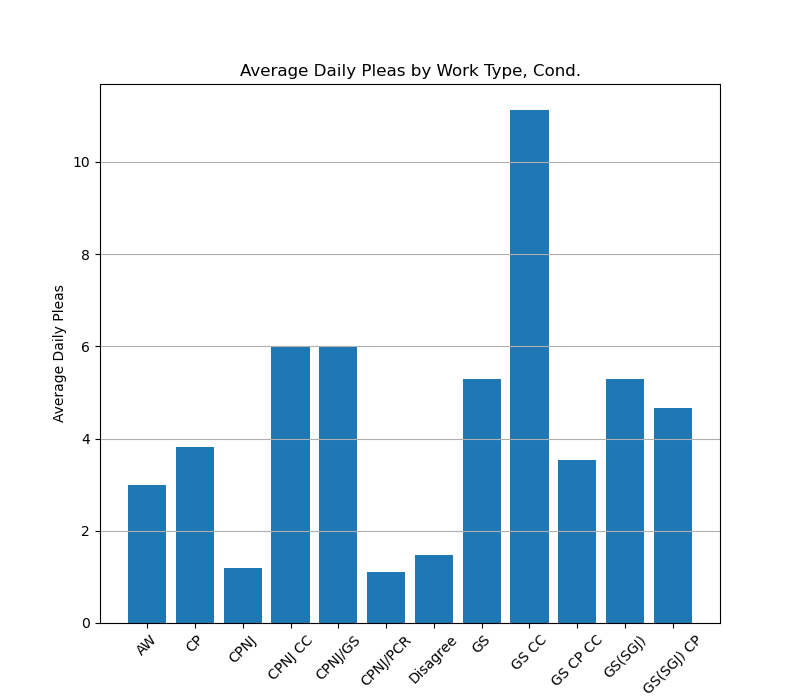
\includegraphics[width=0.75\textwidth]{../../../output/figures/Exploration/avg_pleas_by_worktype_cond.png}
    \caption{Average Pleas Processed per Day by Work Type, conditional on observing at least one sentencing event on that day. Disagree is when the sentencing and schedule data disagree, so we don't know what the work type is.}
    \label{fig-avg-plea-cond}
  \end{figure}

  \begin{figure}[H]
    \centering
    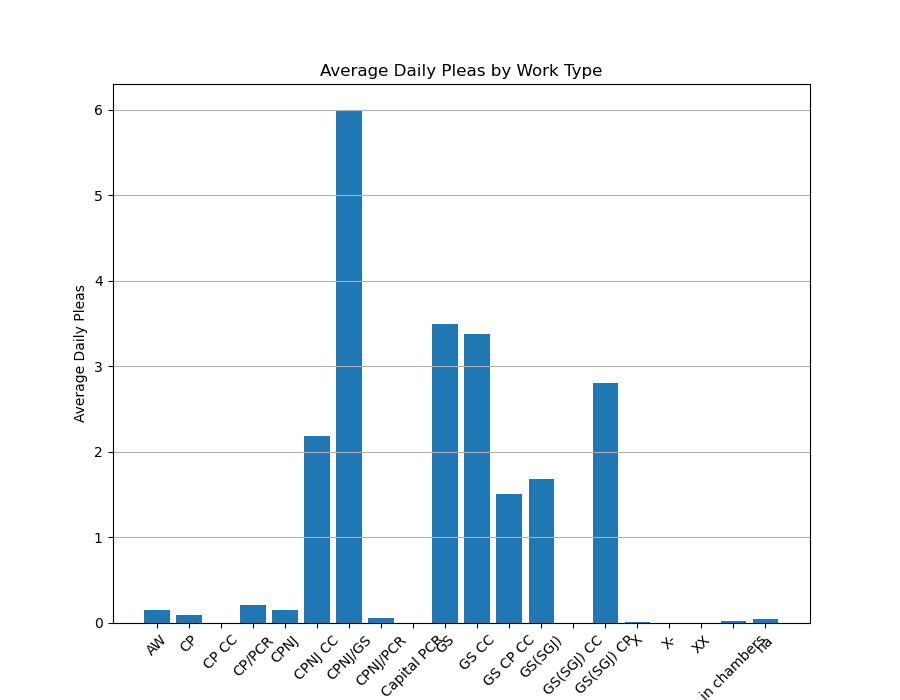
\includegraphics[width=0.75\textwidth]{../../../output/figures/Exploration/avg_pleas_by_worktype.png}
    \caption{Average Pleas Processed per Day by Work Type}
    \label{fig-avg-plea}
  \end{figure}

\section{Discussion about what to do with missing dates}
  Similarly, I wanted to have a better idea of the distribution of missing days across judges and counties. I also wanted to know if the fraction of events missing dates varied considerably across judges. I also used the method described in Nasser's document to recover the dates for 99 of the events with missing dates. I then plotted the distribution of the dates of these events in Figure \ref{fig-missing-month} to check if events with missing dates appeared to be clustered in a specific month. Note, all judges have at least one sentencing event with a missing date.

  \begin{figure}[H]
    \centering
    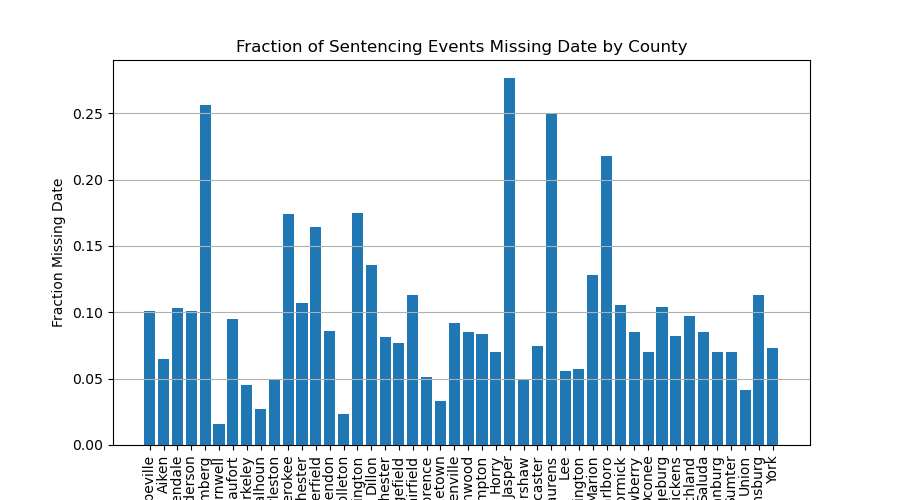
\includegraphics[width=0.85\textwidth]{../../../output/figures/Exploration/fraction_missing_date_by_County.png}
    \caption{Fraction of events missing dates by county}
    \label{fig-frac-missing-county}
  \end{figure}

  \begin{figure}[H]
    \centering
    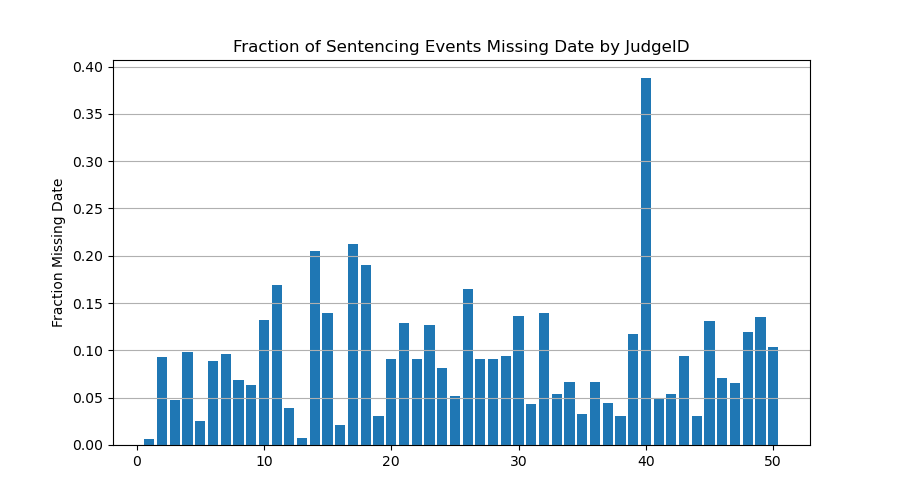
\includegraphics[width=0.85\textwidth]{../../../output/figures/Exploration/fraction_missing_date_by_JudgeID.png}
    \caption{Fraction of events missing dates by judge}
    \label{fig-frac-missing-judge}
  \end{figure}

  \begin{figure}[H]
    \centering
    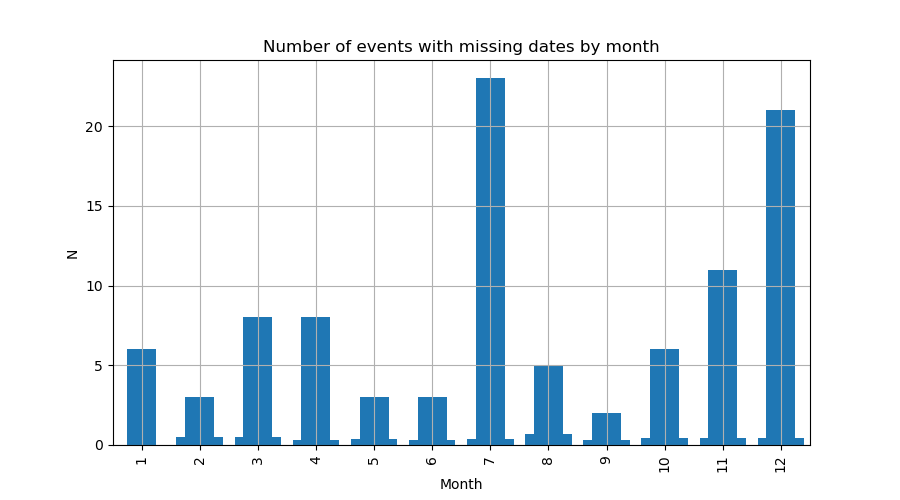
\includegraphics[width=0.65\textwidth]{../../../output/figures/Exploration/missing_date_month_hist.png}
    \caption{Distribution of missing date events by month}
    \label{fig-missing-month}
  \end{figure}

\section{Implementation of Convex Hull Approach}
  I finished implementing the convex hull approach for the minimum and maximum plea as you described. As a reminder, given $\theta \tau$ and the simplices of the judge's convex hull, we first find the two line segments in which $\theta \tau$ lies, and then we find the value of the convex hull at $\theta \tau$ in each of those two line segments using linear interpolation. The maximum and minimum of these two values will be the maximum and minimum plea for that $\theta \tau$.
  We still have to figure out what to do if $\theta \tau$ is not in the domain of the convex hull.

  \begin{figure}[H]
    \centering
    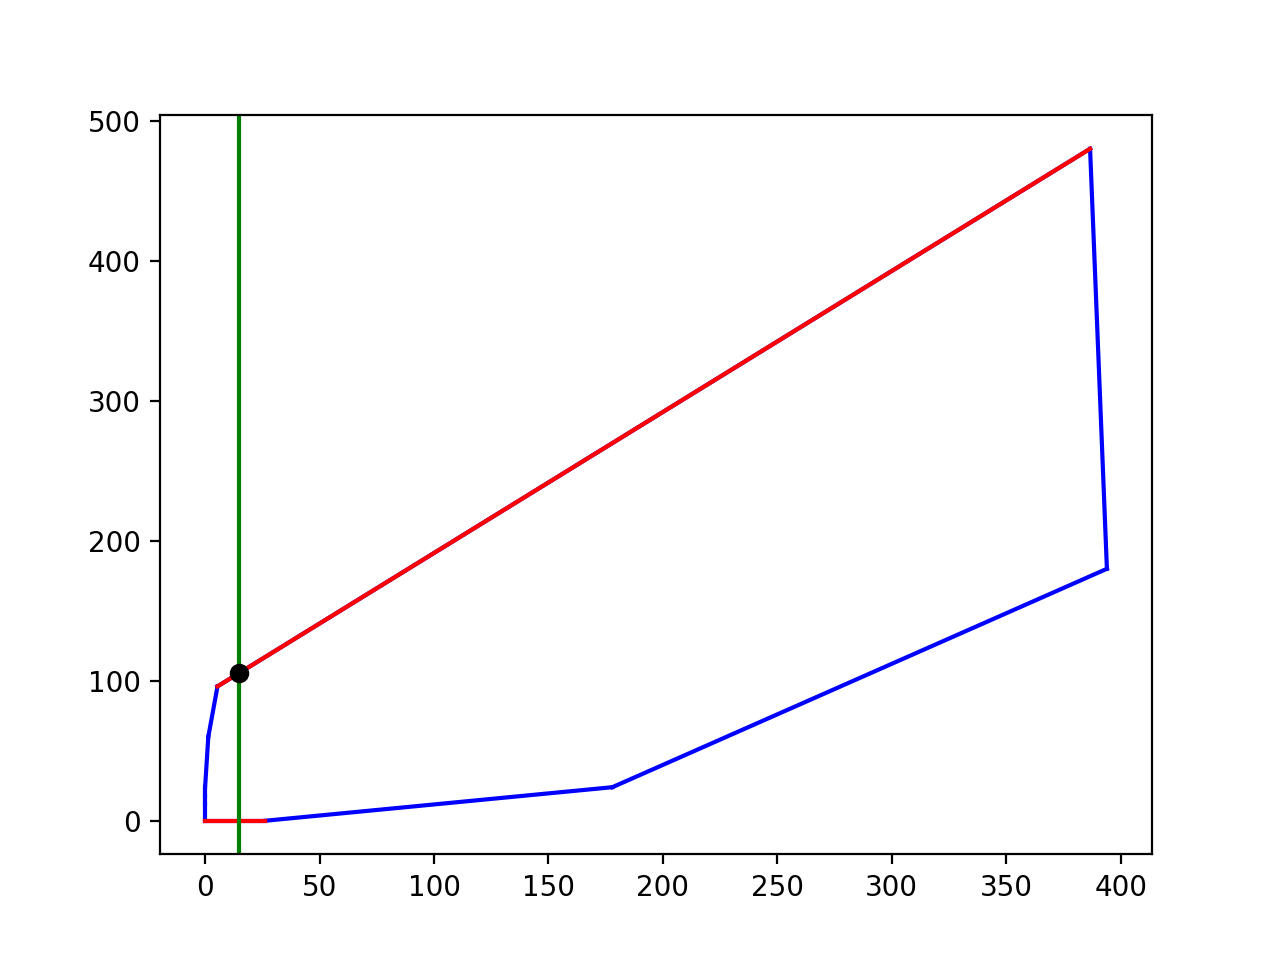
\includegraphics[width=0.65\textwidth]{../../../output/figures/Exploration/convex_hull_max.png}
    \caption{Example of convex hull approach. The convex hull is in blue, the two line segments containing $\theta \tau$ are in red, and the green line intercepts the x-axis at $\theta \tau$. The black dot would be the maximum plea.}
    \label{fig-convex-hull}
  \end{figure}

\section{Trial Scheduling in the Simulation}
  We first describe a method to assign a set of judges to a set of counties for T time periods. The time periods here are discrete and we think of them as weeks. We describe how the assignment would work for each individual week, but in practice all the assignments would be determined before running the rest of the simulation. Since there are 50 judges and 46 counties, in each period we would randomly draw, without replacement, 46 judges from the list of 50. Then, each of the selected judges will stay in his "home" county with probability $\eta$ and with probability $1-\eta$ he will be assigned to another county. We refer to judges that don't stay in their home county in a specific week as "rotating judges", and we refer to counties whose home judge will be rotating as "rotating counties". We assign rotating judges to rotating counties as follows: we randomly shuffle the rotating judges and the rotating counties are sorted alphabetically. So the rotating judge in the first position after shuffling would be assigned to county A, the second to County B, and so on.

  \subsection{Option 1}
    In the first option for scheduling trials would be as follows. We would first assign judges to counties using the method described above. Then, suppose that for a specific judge, $j$, we want to schedule $n$ trials. Suppose that each trial takes 2 weeks to process, and let $m$ be the number of times that $j$ is assigned to the same county on two consecutive weeks. We would assign the trials by randomly choosing $n$ of the $m$ times that a judge is assigned to the same county on two consecutive weeks. Then, for those two weeks, the judge would have no capacity.

    \paragraph{Example}
    For a more concrete example, look at Table \ref{tab:op1}. Suppose that we already ran the procedure for assigning judges to counties and that table \ref{tab:op1} contains the assignments for judges 1 and 2. Suppose that we want to schedule 1 trial for judge 1. There are two times in judge 1's schedule where he is in the same county in two consecutive time periods, one of these times starts in period 1, and the other in period 6. To schedule judge 1's trial, we would randomly choose 1 2-period block from periods 1-2 and periods 6-7. Suppose we choose periods 1-2, then judge 1's capacity for periods 1-2 would be 0.

    \begin{table}[H]
      \centering
      \caption{Option 1 Judge Assignments}
      \label{tab:op1}
      \begin{tabular}{lllllllll}
                       & \textbf{1} & \textbf{2} & \textbf{3} & \textbf{4} & \textbf{5} & \textbf{6} & \textbf{7} & \textbf{8} \\
      \textbf{Judge 1} & Horry      & Horry      & Aiken      & Greenville & Marion     & York       & York       & Union      \\
      \textbf{Judge 2} & Marion     & Aiken      & Aiken      & Horry      & Marion     & Kershaw    & Horry      & Horry
      \end{tabular}
    \end{table}


  \subsection{Option 2}
    Suppose that for a specific judge, $j$, we want to schedule $n$ trials. Suppose that each trial takes 2 weeks to process. For judge $j$, we would first divide his schedule into two week blocks. For example, periods 1 and 2 would become period 1, periods 3-4 would become period 2 and so on. If there are initially $T$ time periods, after doing this we will have $T/2$ time periods. After dividing his schedule into two week blocks, we would randomly select $n$ of these two week blocks and assign the judge to sit in his home county during those blocks and eliminate his capacity for those any two week block that was chosen. Following this, each week some counties and judges will already have assignments. We can use the method described above to assign the remaining judges to the remaining counties.

    \paragraph{Example}
    For a more concrete example consider Table \ref{tab:first-sched}. Suppose that we want to schedule 1 trial for judge 1 and that judge 1's home county is Horry. We would choose one two-period block from (1-2,3-4,5-6,7-8). Suppose we chose block 1-2. Judge 1 will then be assigned to Horry for those two time periods because that is his home county, furthermore, his capacity in those two weeks will be zero. Suppose that using a similar procedure, we assigned 1 trial for Judge 2 in the block 7-8 and that judge 2's home county is Aiken. The judges' schedules following that would look like Table \ref{tab:first-sched}. The county schedules would look like Table \ref{tab:county-sched}. Note that after this initial assignment, each period there will be some counties with no assigned judges. We can assign the remaining judges to these remaining counties using the method described above.

    \begin{table}[H]
      \centering
      \caption{Option 2 judge schedules}
      \label{tab:first-sched}
      \begin{tabular}{lllllllll}
                       & \textbf{1} & \textbf{2} & \textbf{3} & \textbf{4} & \textbf{5} & \textbf{6} & \textbf{7} & \textbf{8} \\
      \textbf{Judge 1} & Horry      & Horry      &            &            &            &            &            &            \\
      \textbf{Judge 2} &            &            &            &            &            &            & Aiken      & Aiken
      \end{tabular}
    \end{table}

    \begin{table}[H]
      \centering
      \caption{Option 2 county schedules}
      \label{tab:county-sched}
      \begin{tabular}{lllllllll}
                     & \textbf{1} & \textbf{2} & \textbf{3} & \textbf{4} & \textbf{5} & \textbf{6} & \textbf{7} & \textbf{8} \\
      \textbf{Horry} & Judge 1          & Judge 1          &            &            &            &            &            &            \\
      \textbf{Aiken} &            &            &            &            &            &            & Judge 2          & Judge 2
      \end{tabular}
    \end{table}

\end{document}
